
\section{Monarch: Definition \& Algorithms}
\label{sec:theory}

In \cref{subsec:parametrization}, we introduce \emph{Monarch matrices},
and describe how they relate to butterfly matrices. In \cref{subsec:ee} we show that the class of Monarch matrices is at least as expressive as the class of butterfly matrices,
while admitting a practically efficient representation.
In particular, many fast transforms (e.g., Fourier, convolution) can be represented as a Monarch matrix or as the product of two or four Monarch matrices (\cref{thm:Monarch_expressiveness}).
In \cref{subsec:projection}, we show how to project onto the set of Monarch
matrices. This allows us to tractably approximate a given matrix
(e.g., a dense pretrained weight matrix) with a Monarch matrix, unlocking new applications~(cf. \cref{sec:experiments}).
In \cref{subsec:recovery}, we show how to recover the individual factors of the
larger class of products of two Monarch matrices.

\subsection{Monarch Parametrization for Square Matrices}
\label{subsec:parametrization}

Inspired by the 4-step FFT algorithm~\citep{bailey1990ffts}, we propose
the class of Monarch matrices, each 
parametrized as the product of two block-diagonal matrices up to permutation:
\begin{definition}\label{def:Monarch}
  Let $n = m^2$. An $n \times n$ \emph{Monarch matrix} has the form:
  \begin{equation*}
    \vM = \vP \vL \vP^\top \vR,
  \end{equation*}
  where $\vL$ and $\vR$ are block-diagonal matrices, each with $m$ blocks of
  size $m \times m$, and $\vP$ is the permutation that maps
  $[x_1, \dots, x_n]$ to
  $[x_1, x_{1+m}, \dots, x_{1+(m-1)m}, x_2, x_{2+m}, \dots, \newline x_{2+(m-1)m}, \dots, x_{m}, x_{2m}, \dots, x_n]$.
\end{definition}
We call this the \emph{Monarch parametrization}. We denote the class of all
matrices that can be written in this form as $\M\ind{n}$ (dropping the superscript when clear from context).
\cref{fig:blockdiag_parametrization} illustrates this parametrization.
\begin{figure}[t]
  \centering
  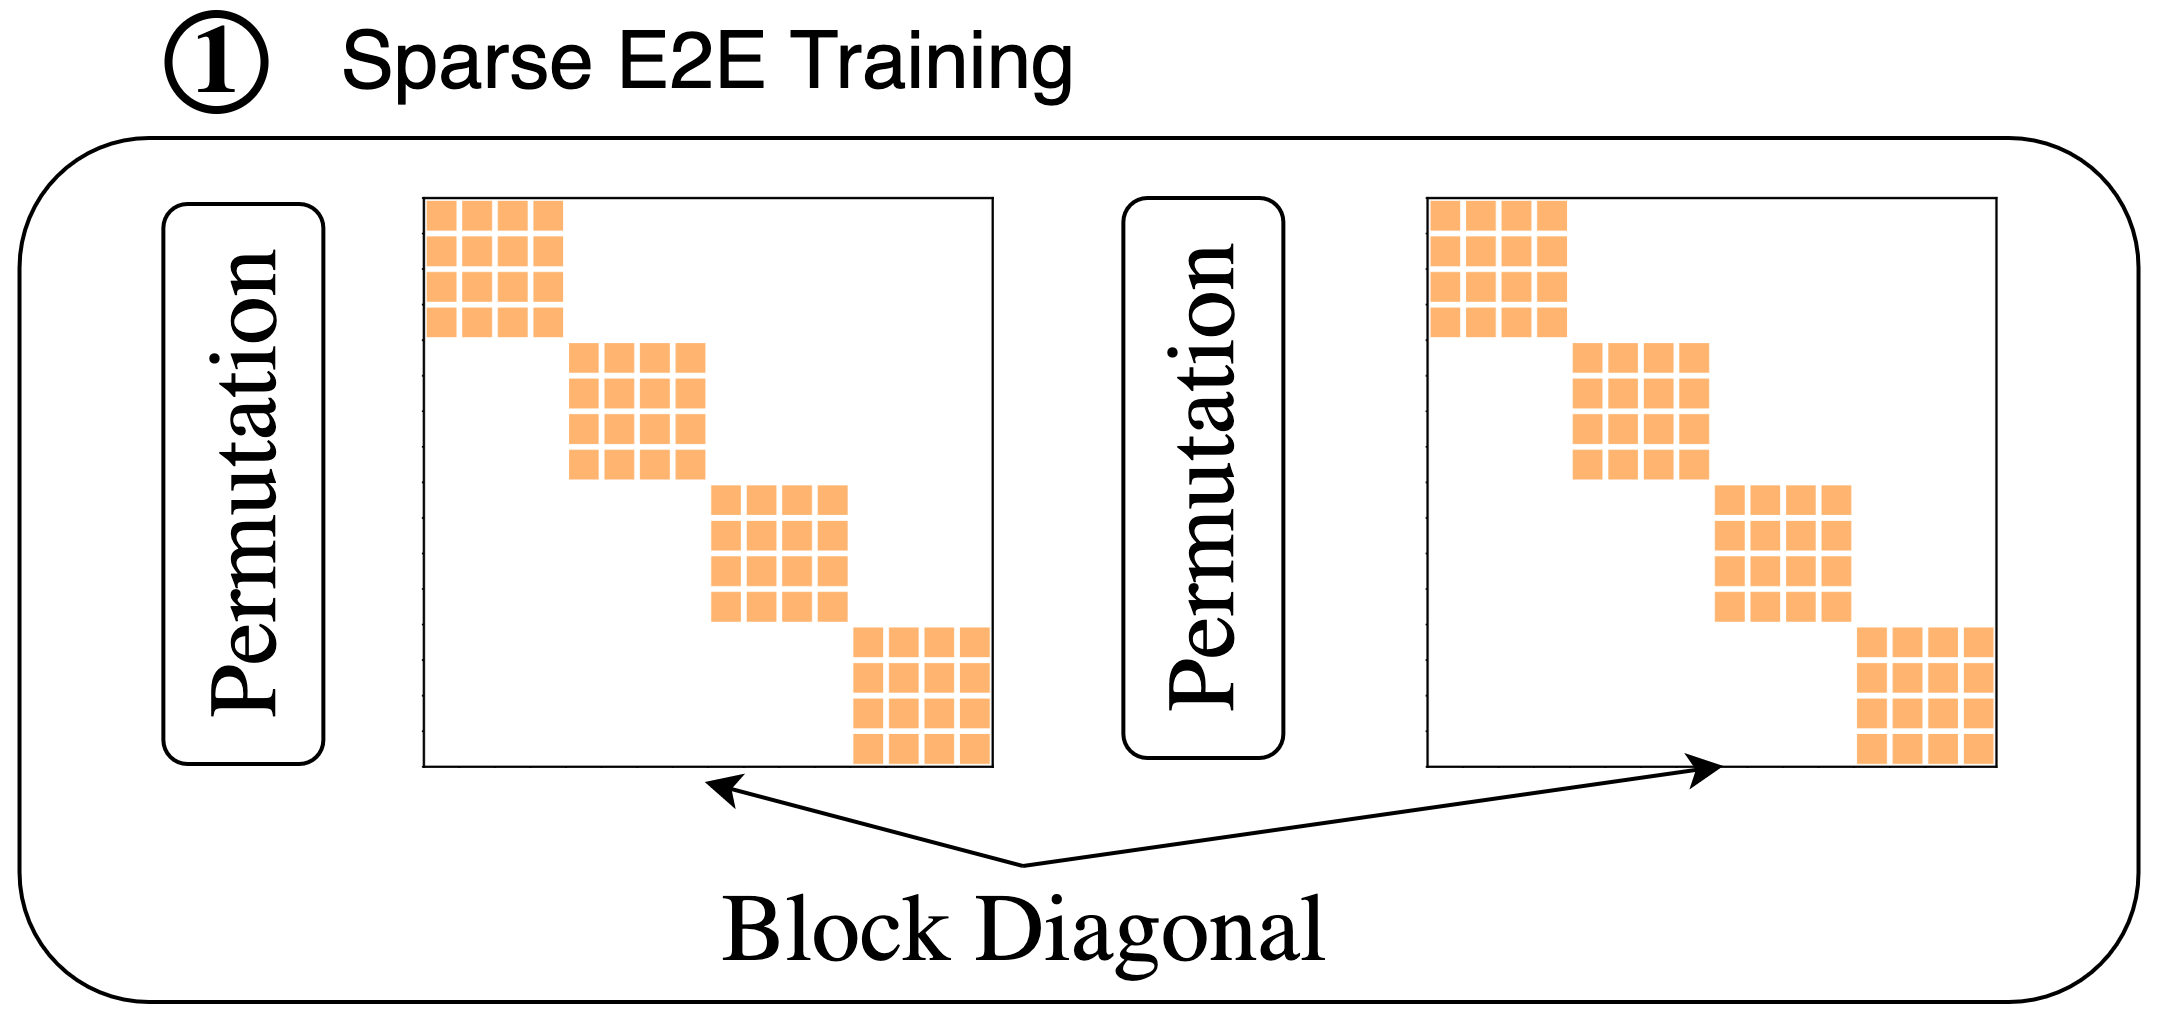
\includegraphics[width=.45\textwidth]{figures/Monarch-1.png}
  \vspace{-1em}
  \caption{\label{fig:blockdiag_parametrization}Monarch matrices are parametrized as products of two block-diagonal
    matrices up to permutation, allowing efficient multiplication algorithm that leverages batch
    matrix multiply.}
  \vspace{-0.5em}
\end{figure}

We now provide more intuition for this parametrization and connect it to butterfly
matrices.
For ease of exposition, suppose $\vB \in \B^{(n)}$ where $n$ is a power of 4.
Then let $\vL'$ be obtained by multiplying together the first $\ff{\log_2 n}{2}$
butterfly factor matrices in the butterfly factorization of $\vB$,
and $\vR$ by multiplying together the last $\ff{\log_2 n}{2}$ butterfly factor matrices.
(We detail this more rigorously in \cref{thm:b_contained}.)

The matrix $\vR$ is block-diagonal with $m = \sqrt{n}$ dense blocks, each block of size
$m \times m$:
$
  \vR = \diag(\vR_1, \dots, \vR_{m}).
$

The matrix $\vL'$ is composed of $m \times m$ blocks of size
$m \times m$, where each block is a diagonal matrix:
\begin{equation*}
  \vL' =
  \begin{bmatrix}
    \vD_{11} & \hdots & \vD_{1m} \\
    \vdots & \ddots & \vdots \\
    \vD_{m1} & \hdots & \vD_{mm} \\
  \end{bmatrix}.
\end{equation*}

The matrix $\vL'$ can also be written as block-diagonal with the same structure as $\vR$
after permuting the rows and columns.
Specifically, let $\vP$ be the permutation of Definition~\ref{def:Monarch}.
We can interpret $\vP$ as follows: it reshapes the vector $x$ of size $n$ as a matrix of size
$m \times m$, transposes the matrix, then converts back into a
vector of size $n$. Note that $\vP = \vP^\top$.
Then we can write
\begin{equation*}
  \vL = \vP \vL' \vP^\top, \quad \text{where } \vL = \diag(\vL_1, \dots, \vL_{m}).
\end{equation*}
Hence, up to permuting rows and columns, $\vL'$ is also a block-diagonal matrix of
$m$ dense blocks, each of size $m \times m$.

Thus we can write $\vB = \vP \vL \vP^\top \vR$,
where $\vL$, $\vR$, and $\vP$ are as in \cref{def:Monarch}.
So, $\vB \in \B\ind{n}$ implies that $\vB \in \M\ind{n}$.

\textbf{Products of Monarch Matrices.}
Another important class of matrices (due to their expressiveness, cf.\ \cref{thm:Monarch_expressiveness})
is the class $\MMS$: matrices that can be written as $\vM_1\vM_2^*$ for some $\vM_1, \vM_2 \in \M$. Further, $(\MMS)^2$ denotes the class of matrices that can be written $\vM_1\vM_2$ for $\vM_1, \vM_2 \in \MMS$.

\textbf{Extension to Rectangular Matrices.}
In practice, we also want a way to parametrize rectangular weight matrices, and to
increase the number of parameters of Monarch matrices to fit different
applications (analogous to the rank parameter in low-rank matrices and the
number of nonzeros in sparse matrices).
We make the simple choice to increase the block size of the block-diagonal
matrices in the Monarch parametrization, and to allow rectangular blocks. More details are in \cref{sec:permutation}.


\subsection{Expressiveness and Efficiency}
\label{subsec:ee}
We remark on the expressiveness of Monarch matrices and their products (ability
to represent many structured transforms), and on their computational and memory efficiency. 
\subsubsection{Expressiveness}
As described in Section \ref{subsec:parametrization}, any matrix $\vB \in \B\ind{n}$ can be written in the Monarch butterfly
representation, by simply condensing the $\log_2 n$ total factors into two matrices.
Thus, the Monarch butterfly representation is strictly more general than the original
butterfly representation (as there also exist matrices in $\M\ind{n}$ but not $\B\ind{n}$).
In other words, for a given size $n$, $\M \supset \B$; similarly $\MMS \supset \BBS$. 
In particular, \citet{dao2020kaleidoscope} showed that the following matrix classes are contained in $\BBS$,
which implies they are in $\MMS$ as well:
\begin{proposition}\label{thm:Monarch_expressiveness}
  The matrix class $\MMS$ can represent convolution, Hadamard
  transform, Toeplitz matrices~\citep{gray2006toeplitz}, and AFDF
  matrices~\citep{moczulski2015acdc}.
  The matrix class $(\MMS)^2$ can represent the Fourier transform, discrete sine and cosine
  transforms (DST/DCT), the $(HD)^3$~\citep{yu2016orthogonal} class,
  Fastfood~\citep{le2013fastfood}, and ACDC matrices~\citep{moczulski2015acdc}.
\end{proposition}



\subsubsection{Efficiency}
\textbf{Parameters.} A Monarch matrix $\vM = \vP\vL\vP^\top \vR$ is described by $2 n \sqrt{n}$ parameters:
$\vL, \vR$ both have $\sqrt{n}$ dense blocks of size $\sqrt{n} \times \sqrt{n}$, for a total
parameter count of $n\sqrt{n}$ each. The permutation $\vP$ is \emph{fixed}, and thus doesn't add any parameters.
\textbf{Speed.}
To multiply by $\vM$, we need to multiply by a block diagonal matrix $\vR$, permute,
multiply by a block diagonal matrix $\vL$, and finally permute.
All four of these steps can be implemented efficiently.
The total number of FLOPs is $O(n \sqrt{n})$, which is more the $O(n \log n)$ for
a butterfly matrix.
However, since we can leverage efficient block-diagonal multiplication (e.g.,
batch matrix multiply), Monarch multiplication is easy to
implement and is fast in practice (2x faster than dense multiply, cf.\ \cref{sec:experiments}).

\subsection{Projection on the Set $\M$ of Monarch Matrices}
\label{subsec:projection}

Given our class of structured matrices, a natural question is the
\emph{projection} problem: finding a Monarch matrix that is the closest to a
given dense matrix.
We show that this problem has an analytical optimal solution, and show how to compute it efficiently.
This allows us to project dense models to Monarch models, enabling D2S
fine-tuning (\cref{subsec:finetuning}).

We formalize the problem: for a given matrix $\vA$, find
\begin{equation}
  \label{eq:projection_objective}
  \argmin\limits_{\vM \in \mathcal{M}} \norm{\vA - \vM}^2_F.
\end{equation}

Even though this problem is nonconvex (as $\vM$ is parametrized as the product of
two matrices), in Theorem~\ref{thm:Monarch_projection} we
show that there exists an analytical solution (full proof in~\cref{sec:proofs}).
This is analogous to the Eckart-Young theorem that establishes that
optimal low-rank approximation is obtained from the SVD~\citep{eckart1936approximation}.
\begin{theorem}\label{thm:Monarch_projection}
  Given an $n \times n$ matrix $\vA$, there is an $O(n^{5/2})$-time algorithm
  that optimally solves the projection problem~\eqref{eq:projection_objective},
  and returns the Monarch factors $\vL$ and $\vR$.
\end{theorem}

We now derive this algorithm (\cref{alg:project}) by examining the structure of
a Monarch matrix $\vM$.

We first rewrite the steps of Monarch matrix-vector multiplication (i.e., computing $\vM \vx$).
The main idea is to view the input $\vx$, which is a vector of size $n = m^2$, as a 2D
tensor of size $m \times m$.
Then the two matrices $\vL$ and $\vR$ in the Monarch parametrization $\vM = \vP\vL\vP^\top \vR$ correspond
to batched matrix multiply along one dimension of $\vx$, followed by batched matrix
multiply along the other dimension of $\vx$.
Thus we view $\vx$ as a 2D tensor of size $m \times m$, and each of
$\vL$ and $\vR$ as a 3D tensor of size $m \times m \times m$.

Steps to multiply $\vx$ by a Monarch matrix $\vM = \vP \vL \vP^\top \vR$:
\begin{enumerate}[leftmargin=*,nosep,nolistsep,noitemsep]
  \item Multiply $\vR$ by $\vx$: $y_{kj} = \sum_i R_{kji} x_{ki}$, to obtain an output $\vy$ that is a
  2D tensor of size $m \times m$.
  \item Multiply $\vP \vL \vP^\top$ by $\vy$: $z_{\ell j} = \sum_k L_{j\ell k} y_{kj}$, to obtain an output
  that is a 2D tensor of size $m \times m$.
  \item Reshape $\vz$ back into a vector of size $n$, and return this.
\end{enumerate}
We can thus write the output $\vz$ as $z_{\ell j} = \sum_{k, i} L_{j\ell k} R_{kji} x_{ki}$.
\newline Since $\vM = \vP \vL \vP^\top\vR$, we can write:
\begin{equation}
  \label{eq:b_einsum}
  M_{\ell jki} = L_{j\ell k} R_{kji}.
\end{equation}
Note that here we view $\vM$ as a 4D tensor of size
$m \times m \times m \times m$.

When viewed as a 4D tensor, the structure of the matrix $\vM$ becomes
apparent, and the solution to the projection problem is easy to see.
Let's examine \cref{eq:b_einsum}: $M_{\ell jki} = L_{j\ell k} R_{kji}$.
We see that this reshaped tensor version of $\vM$ is simply $m \cdot m$ batches of
rank-1 matrices: we batch over the dimensions $k$ and $j$, and each batch is
simply a rank-1 matrix $(\vp_{jk}) (\vq_{jk})^\top$ for some length-$m$ vectors $\vp_{jk}, \vq_{jk}$.

Therefore, the projection objective (\cref{eq:projection_objective}) can be broken up
into the sum of $m \cdot m$ independent terms, each term corresponding to a
block of $\vA$ of size $m \times m$.
As the structure of a Monarch matrix forces each
block to have rank 1 as described above,
the solution to the projection problem becomes apparent:
given a matrix $\vA$, reshape it to a 4D tensor of size
$m \times m \times m \times m$, and take the rank-1
approximation of each batch with the SVD, which (after reshaping)
yields the factors $\vL, \vR$ of the desired matrix $\vM \in \mathcal{M}$.
(Note that if $\vA \in \M$ itself, this algorithm recovers the factors such that $\vA = \vP \vL \vP^\top\vR$.)


\begin{algorithm}[H]
  \caption{\label{alg:project}Projection on the set of Monarch matrices}
  \begin{algorithmic}
    \REQUIRE Matrix $\vA \in \R^{n \times n}$, with $n = m^2$.
    \STATE Reshape $\vA$ into a 4D tensor $\widetilde{\vA}$ of size $m \times m \times m \times m$, where
    $\widetilde{\vA}_{\ell jki} = \vA_{(\ell - 1) m + j, (k-1)m + i}$ for $\ell, j, k, i = 1, \dots, m$.\\
    \FOR{$1 \le j, k \le m$}
    \STATE Let $\widetilde{\vM}_{jk} = \widetilde{\vA}_{:, j, k, :}$ of size $m \times m$.
    \STATE Compute the best rank-1 approximation of $\widetilde{\vM}_{jk}$ as $\vu_{jk} \vv_{jk}^\top$ with the SVD of $\widetilde{\vA}$.
    \ENDFOR
    \STATE Let $\widetilde{\vR}$ be the $m \times m \times m$ tensor where $\widetilde{\vR}_{kji} = (\vv_{jk})_i$.
    \STATE Let $\widetilde{\vL}$ be the $m \times m \times m$ tensor where $\widetilde{\vL}_{j \ell k} = (\vu_{jk})_\ell$.
    \STATE Return $\widetilde{\vL}$, $\widetilde{\vR}$ as block-diagonal matrices $\vL, \vR$ (where the $b^{th}$ block of $\vL,\vR$ are $\widetilde{\vL}_{b,:,:}$, $\widetilde{\vR}_{b,:,:}$ respectively)
  \end{algorithmic}
\end{algorithm}

\subsection{Factorization of $\MMS$ Matrices}
\label{subsec:recovery}
In the previous section, we saw how to project onto the set $\M$.
As Theorem~\ref{thm:Monarch_expressiveness} shows, the broader class $\MMS$ also encompasses many important linear transforms.
In this section, we present an algorithm to compute the Monarch factorization of a given matrix $\vM \in \MMS$, under mild assumptions.
This allows us to store and apply $\vM$ efficiently.



\begin{figure}[t]
  \centering
  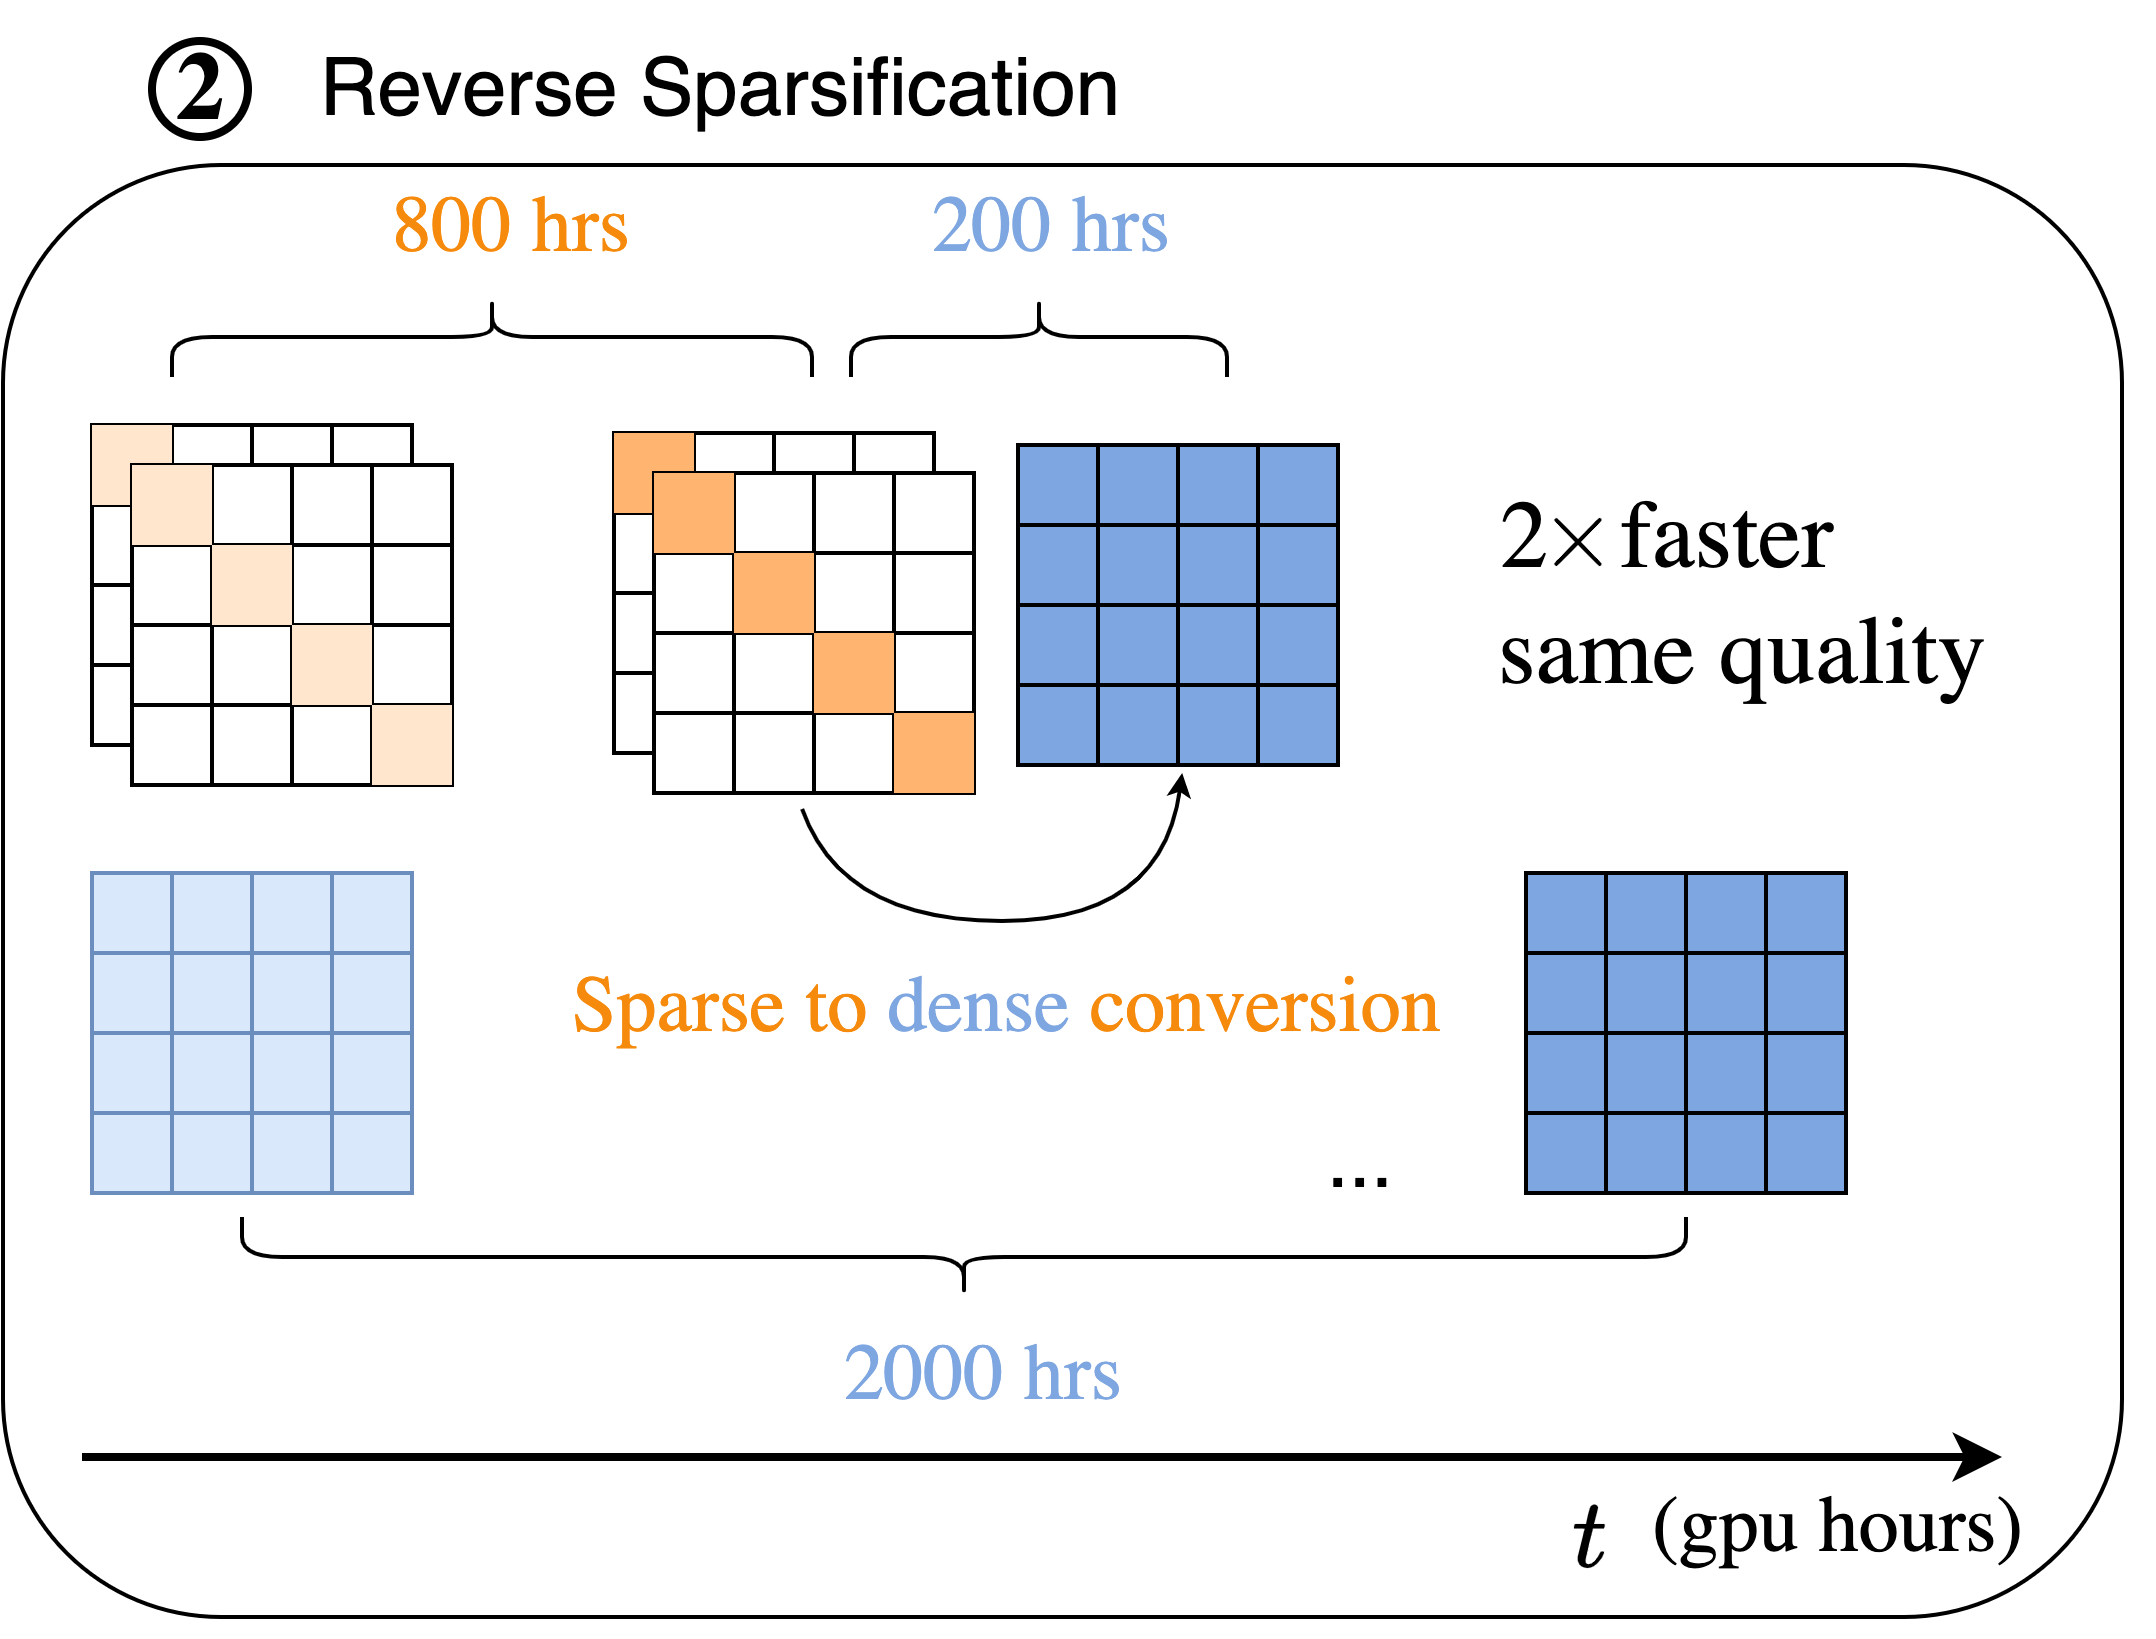
\includegraphics[width=.4\textwidth]{figures/Monarch-2.png}
  \vspace{-0.5em}
  \caption{\label{fig:reverse_sparsification}With the ``reverse sparsification'' process, Monarch matrices can speed up GPT-2 training by 2x.}
  \vspace{-0.5em}
\end{figure}



Specifically, observe that if $\vM \in \MMS$, we can write $\vM = (\vP\vL \vP^\top \vR) (\vR'^* \vP\vL'^* \vP^\top) = (\vP\vL_1\vP^\top) \vR (\vP\vL_2\vP^\top)$ for block-diagonal $\vL_1,\vL_2,\vR$ and the permutation $\vP$ of \cref{def:Monarch}.
Then, we can compute $\vL_1,\vL_2,\vR$ in such a factorization under Assumption \ref{assump:a1}, as stated in \cref{thm:Monarch_recovery}.  (Note that the factorization is not unique.)
\begin{assumption}
\label{assump:a1}
Assume that (1) $\vM \in \MMS$ is invertible and (2) $\vM$ can be written as $(\vP\vL_1\vP^\top)\vR(\vP\vL_2\vP^\top)$ where the blocks of $\vR$ have no zero entries.%
\end{assumption}%

\begin{theorem}\label{thm:Monarch_recovery}
Given an $n \times n$ matrix $\vM \in \MMS$ satisfying Assumption \ref{assump:a1}, there is an $O(n^{5/2})$-time algorithm to find its Monarch factors $\vL_1, \vR, \vL_2$.
\end{theorem}

\mbox{To understand how to do this, define $\tilde{\vM} = \vP^\top \vM\vP$} \mbox{and observe that $\tilde{\vM}\, = \, \vL_1 (\vP\vR\vP^\top) \vL_2 \, =$} \newline
{
\setstretch{0.67}
\setlength\arraycolsep{1.2pt}
${}\hspace{-0.35em}\small \lt \begin{array}{ccccc} \vA_1 \\ & \vA_2 \\ & & \ddots \\ & & & \vA_{m} \end{array}\rt
\lt \begin{array}{cccc} \vD_{11} & \vD_{12} & \dots & \vD_{1m} \\ \vD_{21} & \vD_{22} & \dots & \vD_{2m} \\ \ddots & \ddots & \ddots & \ddots  \\ \vD_{m1} & \vD_{m2} & \dots & \vD_{mm} \end{array}\rt
\lt \begin{array}{ccccc} \vC_1 \\ & \vC_2 \\ & & \ddots \\ & & & \vC_{m} \end{array}\rt$
}

where $m = \sqrt{n}$, the $\vA_i$'s and $\vC_j$'s denote the $m \times m$ diagonal blocks of $\vL_1,\vL_2$ respectively, and each $\vD_{ij}$ is an $m \times m$ diagonal matrix. If we write $\MM$ as a block matrix with $m \times m$ blocks each of size $m \times m$, then we see that the block $\MM_{ij}$ is equal to $\vA_i \vD_{ij} \vC_j$. Notice that $\vM$ is invertible only if all the $\vA_i$'s and $\vC_j$'s are (since if any one of these is singular, then $\vL_1$ or $\vL_2$ is singular).

Thus, our goal is to find matrices $\hat{\vA}_1,\dots,\hat{\vA}_m, \hat{\vC}_1,\dots,\hat{\vC}_m$ and \emph{diagonal} matrices $\hat{\vD}_{11},\dots,\hat{\vD}_{mm}$ such that $\MM_{ij} = \hat{\vA}_i \hat{\vD}_{ij} \hat{\vC}_j$ for all $i,j$; this represents a valid Monarch factorization of $\vM$.

To provide intuition for how to do this, let's analyze a simple case in which all the $\vD_{ij}$'s are the identity matrix. Then we have the set of equations $\vA_i \vC_j = \MM_{ij}$. Again assume the $\vA_i$'s and $\vC_j$'s are invertible, so each $\MM_{ij}$ is as well. Suppose we set $\hat{\vC}_1 = \vI$ (identity matrix). Then we can immediately read off $\hat{\vA}_i = \MM_{i1}$ for all $i$. We can then set $\hat{\vC}_j = \hat{\vA}_1^{-1}\MM_{1j}$ for all $j$.
Let's now check that this strategy gives a valid factorization, i.e., that $\MM_{ij} = \hat{\vA}_i \hat{\vC}_j$ for all $i,j$. We have $\hat{\vA}_i \hat{\vC}_j = \MM_{i1} \MM_{11}^{-1} \MM_{1j}$. Recalling that in the ``true'' factorization we have $\MM_{ij} = \vA_i \vC_j$, this equals $(\vA_i \vC_1) (\vA_1 \vC_1)^{-1} (\vA_1 \vC_j) = \vA_i \vC_j$, as desired.



In the general case, we must deal with the diagonal $\vD_{ij}$ matrices as well. We will no longer be able to freely set $\hat{\vC}_1 = \vI$. However, once we find a proper choice of $\hat{\vC}_1$, we can use it to find all the $\hat{\vA}_i$'s and $\hat{\vC}_j$'s. We can find such a $\hat{\vC}_1$ via the idea of \emph{simultaneous diagonalization}; for space reasons,
we defer a full description of our algorithm (\cref{alg:mm_recovery}), and its analysis, to Appendix \ref{sec:proofs}.






\begin{figure}[t]
  \centering
  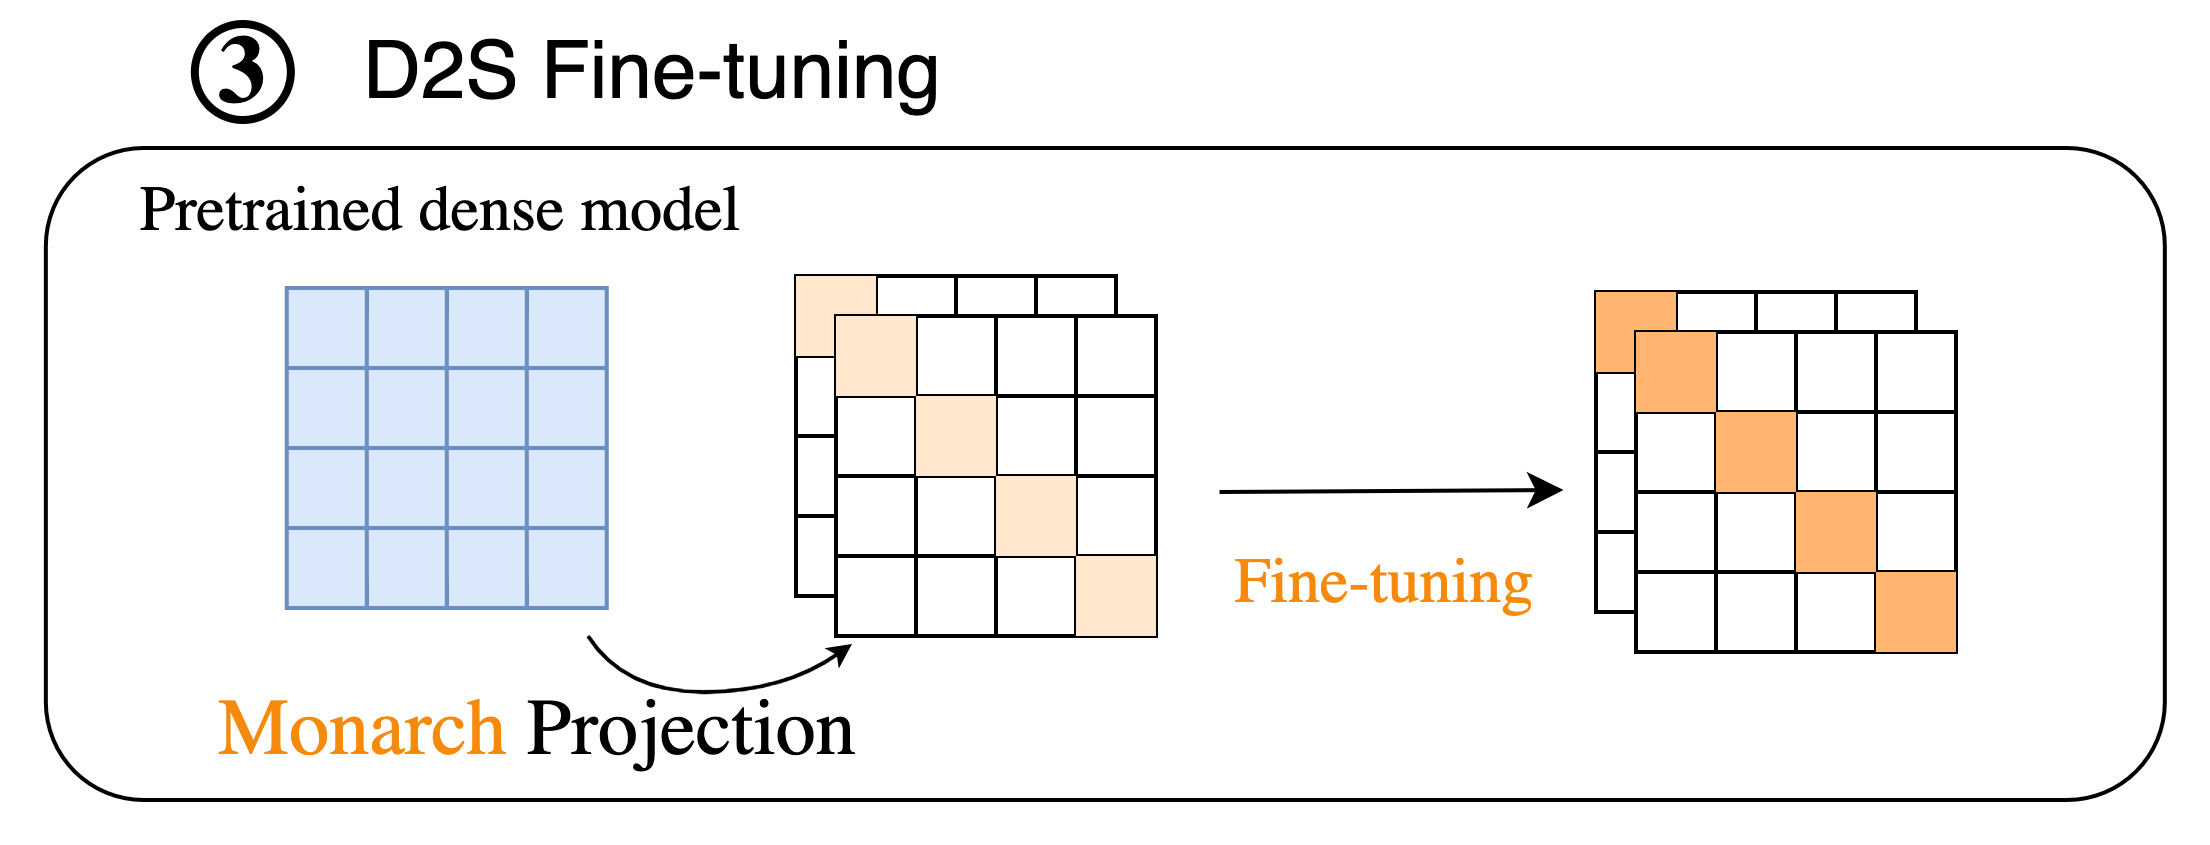
\includegraphics[width=.45\textwidth]{figures/Monarch-3.png}
  \vspace{-1em}
  \caption{\label{fig:monarch_projection}With~\cref{alg:project} for our Monarch parameterization, we can convert a pretrained model into a model with Monarch weight matrices and speed up downstream fine-tuning.}
  \vspace{-1.0em}
\end{figure}


